% Problems, Chapter 1: Introduction to Electrostatics
% Jackson, Classical Electrodynamics, 3rd ed.
% Requires: amsmath, amssymb, tikz

\section*{Problems}

\Needspace{5\baselineskip}
\par\bigskip
\noindent\textbf{1.1}\quad Use Gauss's theorem [and (1.21) if necessary] to prove the following:
\begin{enumerate}
\item[(a)] Any excess charge placed on a conductor must lie entirely on its surface. (A conductor by definition contains charges capable of moving freely under the action of applied electric fields.)
\item[(b)] A closed, hollow conductor shields its interior from fields due to charges outside, but does not shield its exterior from the fields due to charges placed inside it. \erratum{For the exterior assertion, take the conductor to be initially neutral and isolated, with a nonzero net charge placed in its cavity.}
\item[(c)] The electric field at the surface of a conductor is normal to the surface and has a magnitude $\erratum{|\sigma|}/\epsilon_{0}$, where $\sigma$ is the charge density per unit area on the surface.
\end{enumerate}
\solution
We assume electrostatic equilibrium, a connected perfect conductor, and vacuum
adjacent to its surface. Let $\mathbf n$ point from the metal into the vacuum.
\begin{enumerate}
\item[(a)] If the field in the metal were nonzero, its mobile charges would
experience $q\mathbf E$ and move. Thus $\mathbf E=0$ there. For every small
volume wholly within the metal,
\[
Q_V=\epsilon_0\oint_{\partial V}\mathbf E\cdot d\mathbf a=0.
\]
Shrinking the volume gives $\rho=0$ in the bulk. Excess charge can therefore
reside only on the boundary. This statement concerns net excess charge, not
the separate positive and negative microscopic charges making up the metal.
\item[(b)] The metal and hence the wall of an empty cavity are at one
potential $V_c$. Put $u=\Phi-V_c$ in the cavity. Green's first identity gives
\[
\int_{\rm cavity}|\nabla u|^2d^3x
=\oint u\,\partial_nu\,da-\int u\nabla^2u\,d^3x=0,
\]
since $u=0$ on the wall and $\nabla^2u=0$ inside. Therefore $u=0$ throughout:
external charges produce no cavity field. This remains a shielding statement
even if fixed charges already occupy the cavity: compare two solutions with
the same interior charges and different exterior sources. Their difference
is harmonic in the cavity and constant on its wall, so the same identity
makes its gradient zero. The interior field therefore does not change.
If a charge $q$ is instead put in
the cavity, a Gaussian surface in the metal enclosing the cavity gives
$0=q+Q_{\rm inner}$, so $Q_{\rm inner}=-q$. An initially neutral, isolated
conductor must then have $Q_{\rm outer}=q$. A Gaussian surface outside the
whole system has flux $q/\epsilon_0$, which is nonzero for $q\ne0$.
The qualification ``isolated'' matters: a grounded closed conductor can draw
$-q$ from ground, leaving no exterior field when there are no exterior sources.
A zero-net-charge interior distribution also need not give an exterior field.
\item[(c)] A narrow rectangular electrostatic loop straddling the surface
has $\oint\mathbf E\cdot d\mathbf l=0$. Letting its height vanish gives
$\mathbf E_{{\rm out},t}=\mathbf E_{{\rm in},t}=0$.
For a pillbox of face area $\Delta a$,
\[
(E_{{\rm out},n}-E_{{\rm in},n})\Delta a
=\frac{\sigma\Delta a}{\epsilon_0}.
\]
Since the interior field vanishes,
$\boxed{\mathbf E_{\rm out}=(\sigma/\epsilon_0)\mathbf n}$.
Its magnitude is $|\sigma|/\epsilon_0$; the signed outward component is
$\sigma/\epsilon_0$.
\end{enumerate}


\Needspace{5\baselineskip}
\par\bigskip
\noindent\textbf{1.2}\quad The Dirac delta function in three dimensions can be taken as the improper limit as $\alpha \rightarrow 0$ of the Gaussian function
\[
D(\alpha;\,x,y,z) = (2\pi)^{-3/2}\alpha^{-3}\exp\left[-\frac{1}{2\alpha^{2}}\left(x^{2}+y^{2}+z^{2}\right)\right]
\]
Consider a general orthogonal coordinate system specified by the surfaces $u = {}$constant, $v = {}$constant, $w = {}$constant, with length elements $du/U$, $dv/V$, $dw/W$ in the three perpendicular directions. Show that
\[
\delta(\mathbf{x}-\mathbf{x}') = \delta(u-u')\;\delta(v-v')\;\delta(w-w')\cdot UVW
\]
by considering the limit of the Gaussian above. Note that as $\alpha \rightarrow 0$ only the infinitesimal length element need be used for the distance between the points in the exponent.
\solution
Write $h_u=1/U$, $h_v=1/V$, and $h_w=1/W$. At a regular coordinate point
$\mathbf x'$, the distance between neighboring points is
\[
|\mathbf x-\mathbf x'|^2
=h_u'^2(u-u')^2+h_v'^2(v-v')^2+h_w'^2(w-w')^2+O(|\Delta\mathbf u|^3).
\]
Set $\xi_u=h_u'(u-u')/\alpha$, and similarly for $v,w$. The local volume
measure is
\[
d^3x=h_uh_vh_w\,du\,dv\,dw
=\alpha^3[1+O(\alpha)]\,d\xi_u\,d\xi_v\,d\xi_w.
\]
For any continuous test function $f$ of compact support, the Gaussian integral
therefore tends to
\[
\begin{split}
\lim_{\alpha\to0}\int D(\alpha;\mathbf x-\mathbf x')f(\mathbf x)d^3x
&=f(\mathbf x')(2\pi)^{-3/2}
\int_{\mathbb R^3}e^{-(\xi_u^2+\xi_v^2+\xi_w^2)/2}d^3\xi\\
&=f(\mathbf x').
\end{split}
\]
Equivalently, each one-dimensional Gaussian has width
$\alpha/h_u'=\alpha U'$, so its normalization supplies a factor $U'$.
Consequently
\[
\boxed{\delta^3(\mathbf x-\mathbf x')
=U'V'W'\delta(u-u')\delta(v-v')\delta(w-w').}
\]
Unprimed $UVW$ is equivalent because the deltas evaluate it at the primed
point. Integrating this expression with $d^3x=du\,dv\,dw/(UVW)$ explicitly
cancels the Jacobian. At coordinate singularities one uses a regular local
chart or interprets the formula through this integration rule.


\Needspace{5\baselineskip}
\par\bigskip
\noindent\textbf{1.3}\quad Using Dirac delta functions in the appropriate coordinates, express the following charge distributions as three-dimensional charge densities $\rho(\mathbf{x})$.
\begin{enumerate}
\item[(a)] In spherical coordinates, a charge $Q$ uniformly distributed over a spherical shell of radius $R$.
\item[(b)] In cylindrical coordinates, a charge $\lambda$ per unit length uniformly distributed over a cylindrical surface of radius $b$.
\item[(c)] In cylindrical coordinates, a charge $Q$ spread uniformly over a flat circular disc of negligible thickness and radius $R$.
\item[(d)] The same as part (c), but using spherical coordinates.
\end{enumerate}
\solution
The defining check is $\int\rho\,d^3x=Q$ (or charge per unit length $\lambda$).
Let $s$ denote cylindrical radius, to distinguish it from the charge density,
and let $H$ be the Heaviside function.
\begin{enumerate}
\item[(a)] The shell has surface density $Q/(4\pi R^2)$, hence
\[
\boxed{\rho(r,\theta,\phi)=\frac{Q}{4\pi R^2}\delta(r-R).}
\]
Indeed, $\int r^2\delta(r-R)dr=R^2$ and $\int d\Omega=4\pi$.
\item[(b)] The charge per circumference is $\lambda/(2\pi b)$:
\[
\boxed{\rho(s,\phi,z)=\frac{\lambda}{2\pi b}\delta(s-b).}
\]
Integration with $s\,ds\,d\phi$ gives $\lambda$ at every $z$.
\item[(c)] The surface density is $\sigma=Q/(\pi R^2)$, so
\[
\boxed{\rho(s,\phi,z)=\sigma H(R-s)\delta(z).}
\]
Its integral is $\sigma\int_0^R2\pi s\,ds=Q$.
\item[(d)] Since $z=r\cos\theta$ and the disk lies at $\theta=\pi/2$,
\[
\delta(r\cos\theta)=\frac1r\delta(\theta-\pi/2),\qquad r>0.
\]
Thus a spherical-coordinate representation is
\[
\boxed{\rho(r,\theta,\phi)=\frac{Q}{\pi R^2r}
H(R-r)\delta(\theta-\pi/2).}
\]
Multiplication by $r^2\sin\theta\,dr\,d\theta\,d\phi$ leaves
$\sigma r\,dr\,d\phi$, the correct disk measure. The apparent $1/r$
singularity is a coordinate factor and introduces no point charge at the origin.
\end{enumerate}


\Needspace{5\baselineskip}
\par\bigskip
\noindent\textbf{1.4}\quad Each of three charged spheres of radius $a$, one conducting, one having a uniform charge density within its volume, and one having a spherically symmetric charge density that varies radially as $r^{n}$ ($n>-3$), has a total charge $Q$. Use Gauss's theorem to obtain the electric fields both inside and outside each sphere. Sketch the behavior of the fields as a function of radius for the first two spheres, and for the third with $n=-2,\,+2$.
\solution
Spherical symmetry gives $4\pi r^2E_r=Q(<r)/\epsilon_0$. Put
$E_a=Q/(4\pi\epsilon_0a^2)$ and $s=r/a$ (the sketches take $Q>0$).
For the conductor, $Q(<r)=0$ for $r<a$ and $Q$ for $r>a$; therefore
\[
E_r=\begin{cases}0&r<a,\\E_as^{-2}&r>a.\end{cases}
\]
For uniform volume density $\rho_0=3Q/(4\pi a^3)$,
\[
Q(<r)=4\pi\rho_0\int_0^r r'^2dr'=Q(r/a)^3,
\qquad E_r=E_as\quad(r<a).
\]
More generally, put $\rho=Kr^nH(a-r)$. Normalization and enclosed charge give
\[
Q=\frac{4\pi Ka^{n+3}}{n+3},\qquad
K=\frac{(n+3)Q}{4\pi a^{n+3}},\qquad
Q(<r)=Q(r/a)^{n+3}.
\]
Hence
\[
\boxed{E_r=E_a\begin{cases}s^{n+1}&0<r<a,\\s^{-2}&r>a.\end{cases}}
\]
For $n=-2$, the interior field is $E_a/s$; it diverges at the center but has
vanishing enclosed charge as $r\to0$, so there is no additional delta charge.
For $n=2$, it is $E_as^3$. Only the conductor has a jump at $r=a$.
\begin{center}
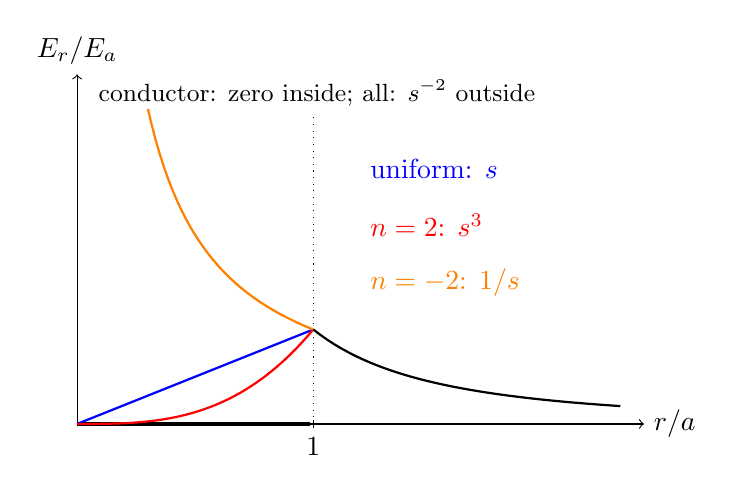
\begin{tikzpicture}[x=3cm,y=1.2cm]
\draw[->] (0,0)--(2.4,0) node[right] {$r/a$};
\draw[->] (0,0)--(0,3.7) node[above] {$E_r/E_a$};
\draw[dotted] (1,0)--(1,3.3);
\draw[black,very thick] (0,0)--(.985,0);
\draw[blue,thick] (0,0)--(1,1);
\draw[red,thick,domain=0:1,samples=40] plot (\x,{\x^3});
\draw[orange,thick,domain=.3:1,samples=45] plot (\x,{1/\x});
\draw[black,thick,domain=1:2.3,samples=45] plot (\x,{1/\x^2});
\draw (1,.04)--(1,-.04) node[below] {$1$};
\node[blue,anchor=west] at (1.2,2.7) {uniform: $s$};
\node[red,anchor=west] at (1.2,2.1) {$n=2$: $s^3$};
\node[orange,anchor=west] at (1.2,1.5) {$n=-2$: $1/s$};
\node[anchor=west,font=\small] at (.05,3.5) {conductor: zero inside; all: $s^{-2}$ outside};
\end{tikzpicture}
\end{center}


\Needspace{5\baselineskip}
\par\bigskip
\noindent\textbf{1.5}\quad The time-averaged potential of a neutral hydrogen atom is given by
\[
\Phi = \frac{q}{4\pi\epsilon_{0}}\frac{e^{-\alpha r}}{r}\left(1+\frac{\alpha r}{2}\right)
\]
where $q$ is the magnitude of the electronic charge, and $\alpha^{-1}=a_{0}/2$, $a_{0}$ being the Bohr radius. Find the distribution of charge (both continuous and discrete) that will give this potential and interpret your result physically.
\solution
For $r>0$, write $\Phi=(q/4\pi\epsilon_0)f(r)$ with
$f=e^{-\alpha r}(1/r+\alpha/2)$. Direct differentiation gives
\[
f'=-e^{-\alpha r}\left(\frac1{r^2}+\frac\alpha r+\frac{\alpha^2}{2}\right),
\quad
(r^2f')'=\frac{\alpha^3r^2}{2}e^{-\alpha r}.
\]
Poisson's equation then yields the continuous part
\[
\rho_c=-\epsilon_0\nabla^2\Phi
=-\frac{q\alpha^3}{8\pi}e^{-\alpha r}\quad(r>0).
\]
The singular part is determined by a small Gaussian sphere:
\[
\lim_{r\to0}4\pi\epsilon_0r^2(-\Phi')=q.
\]
Thus
\[
\boxed{\rho(\mathbf r)=q\delta^3(\mathbf r)
-\frac{q\alpha^3}{8\pi}e^{-\alpha r}.}
\]
Its continuous charge is
$-q\alpha^3\int_0^\infty r^2e^{-\alpha r}dr/2=-q$, since the integral
is $2/\alpha^3$. With $\alpha=2/a_0$,
$\rho_c=-q e^{-2r/a_0}/(\pi a_0^3)$: a point proton plus the mean charge
cloud of a hydrogen $1s$ electron. The total charge is zero, consistently
with the exponentially screened large-$r$ potential.


\Needspace{5\baselineskip}
\par\bigskip
\noindent\textbf{1.6}\quad A simple capacitor is a device formed by two insulated conductors adjacent to each other. If equal and opposite charges are placed on the conductors, there will be a certain difference of potential between them. The ratio of the magnitude of the charge on one conductor to the magnitude of the potential difference is called the capacitance (in SI units it is measured in farads). Using Gauss's law, calculate the capacitance of
\begin{enumerate}
\item[(a)] two large, flat, conducting sheets of area $A$, separated by a small distance $d$;
\item[(b)] two concentric conducting spheres with radii $a$, $b$ ($b>a$);
\item[(c)] two concentric conducting cylinders of length $L$, large compared to their radii $a$, $b$ ($b>a$).
\item[(d)] What is the inner diameter of the outer conductor in an air-filled coaxial cable whose center conductor is a cylindrical wire of diameter 1 mm and whose capacitance is $3\times10^{-11}$ F/m? $3\times10^{-12}$ F/m?
\end{enumerate}
\solution
Take $Q>0$ on the inner/positive conductor and define
$V=\Phi_+-\Phi_->0$. The electrostatic capacitance is $C=Q/V$.
\begin{enumerate}
\item[(a)] A Gaussian pillbox gives $E=Q/(\epsilon_0 A)$ in the gap.
Consequently $V=\int_0^d E\,dz=Qd/(\epsilon_0A)$, and
$\boxed{C=\epsilon_0A/d}$. Edge effects are neglected.
\item[(b)] A Gaussian sphere gives $E_r=Q/(4\pi\epsilon_0r^2)$ for $a<r<b$.
Therefore
\[
V=\frac{Q}{4\pi\epsilon_0}\int_a^b\frac{dr}{r^2}
=\frac{Q}{4\pi\epsilon_0}\left(\frac1a-\frac1b\right),\qquad
\boxed{C=4\pi\epsilon_0\frac{ab}{b-a}}.
\]
\item[(c)] For a coaxial Gaussian cylinder,
$2\pi rLE_r=Q/\epsilon_0$, whence
\[
V=\frac{Q}{2\pi\epsilon_0L}\int_a^b\frac{dr}{r}
=\frac{Q}{2\pi\epsilon_0L}\ln\frac ba,\qquad
\boxed{C=\frac{2\pi\epsilon_0L}{\ln(b/a)}}.
\]
End corrections are negligible when the length is much larger than the radii.
\item[(d)] With $C'=C/L$, $b/a=\exp(2\pi\epsilon_0/C')$. Since $2a=1$ mm,
\[
2b=(1\ {\rm mm})\exp(2\pi\epsilon_0/C')
=\begin{cases}
6.388\ {\rm mm},&C'=3\times10^{-11}\ {\rm F/m},\\
1.1314\times10^5\ {\rm m},&C'=3\times10^{-12}\ {\rm F/m}.
\end{cases}
\]
Here air is approximated by vacuum, $\epsilon_0\simeq8.85419\times10^{-12}$ F/m.
The second value is a formal coaxial result and would require an enormous
outer cylinder and still greater length for the end-free approximation.
\end{enumerate}


\Needspace{5\baselineskip}
\par\bigskip
\noindent\textbf{1.7}\quad Two long, cylindrical conductors of radii $a_{1}$ and $a_{2}$ are parallel and separated by a distance $d$, which is large compared with either radius. Show that the capacitance per unit length is given approximately by
\[
C \simeq \pi\epsilon_{0}\left(\ln\frac{d}{a}\right)^{-1}
\]
where $a$ is the geometrical mean of the two radii.

Approximately what gauge wire (state diameter in millimeters) would be necessary to make a two-wire transmission line with a capacitance of $1.2\times10^{-11}$ F/m if the separation of the wires was 0.5 cm? 1.5 cm? 5.0 cm?
\solution
Let the wire charges per unit length be $+\lambda$ and $-\lambda$.
For a line charge, integrating $E_r=\lambda/(2\pi\epsilon_0r)$ gives
$\Phi(r_2)-\Phi(r_1)=-(\lambda/2\pi\epsilon_0)\ln(r_2/r_1)$.
Superposing the two lines and evaluating at their surfaces, to leading order
in $a_i/d$, gives
\[
\Phi_1=\frac{\lambda}{2\pi\epsilon_0}\ln\frac d{a_1}+\Phi_*,\qquad
\Phi_2=-\frac{\lambda}{2\pi\epsilon_0}\ln\frac d{a_2}+\Phi_*.
\]
Subtracting eliminates the arbitrary constant:
\[
V=\frac{\lambda}{2\pi\epsilon_0}\ln\frac{d^2}{a_1a_2}
=\frac{\lambda}{\pi\epsilon_0}\ln\frac d{\sqrt{a_1a_2}},\qquad
\boxed{C'=\frac{\pi\epsilon_0}{\ln(d/a)},\quad a=\sqrt{a_1a_2}.}
\]
For equal radii and $C'=1.2\times10^{-11}$ F/m,
\[
2a=2d\exp\left(-\frac{\pi\epsilon_0}{C'}\right)=0.19694\,d.
\]
Thus the requested diameters for separations $0.5$, $1.5$, and $5.0$ cm are,
respectively,
\[\boxed{0.985,\ 2.954,\ 9.847\ {\rm mm}.}\]
These diameters specify the required wire size without choosing a national
gauge convention. The ratio $a/d\simeq0.0985$ also shows that the calculation
is approximate rather than an exact finite-radius two-cylinder solution.


\Needspace{5\baselineskip}
\par\bigskip
\noindent\textbf{1.8}\quad\begin{enumerate}
\item[(a)] For the three capacitor geometries in Problem 1.6 calculate the total electrostatic energy and express it alternatively in terms of the equal and opposite charges $Q$ and $-Q$ placed on the conductors \emph{and} the potential difference between them.
\item[(b)] Sketch the energy density of the electrostatic field in each case as a function of the appropriate linear coordinate.
\end{enumerate}
\solution
At an intermediate charge $q$, the voltage is $q/C$. The charging work is
\[
U=\int_0^Q\frac qC\,dq=\frac{Q^2}{2C}=\frac12CV^2=\frac12QV.
\]
For the three geometries this gives
\[
\begin{array}{c|c|c}
 &U(Q)&U(V)\\\hline
\text{planes}&\displaystyle\frac{Q^2d}{2\epsilon_0A}
&\displaystyle\frac{\epsilon_0AV^2}{2d}\\[5pt]
\text{spheres}&\displaystyle\frac{Q^2}{8\pi\epsilon_0}\left(\frac1a-\frac1b\right)
&\displaystyle\frac{2\pi\epsilon_0abV^2}{b-a}\\[5pt]
\text{cylinders}&\displaystyle\frac{Q^2}{4\pi\epsilon_0L}\ln\frac ba
&\displaystyle\frac{\pi\epsilon_0LV^2}{\ln(b/a)}
\end{array}
\]
For part (b), the local energy density is $u=\epsilon_0E^2/2$. Therefore
\[
u=\begin{cases}
Q^2/(2\epsilon_0A^2),&0<z<d\quad\text{(planes)},\\
Q^2/(32\pi^2\epsilon_0r^4),&a<r<b\quad\text{(spheres)},\\
Q^2/(8\pi^2\epsilon_0L^2r^2),&a<r<b\quad\text{(cylinders)}.
\end{cases}
\]
It is zero outside these gaps for the ideal equal-and-opposite capacitor
charges. As an independent check, integrating the spherical density with
$4\pi r^2dr$ gives $Q^2(1/a-1/b)/(8\pi\epsilon_0)$; integrating the
cylindrical density with $2\pi rLdr$ gives $Q^2\ln(b/a)/(4\pi\epsilon_0L)$.
\begin{center}
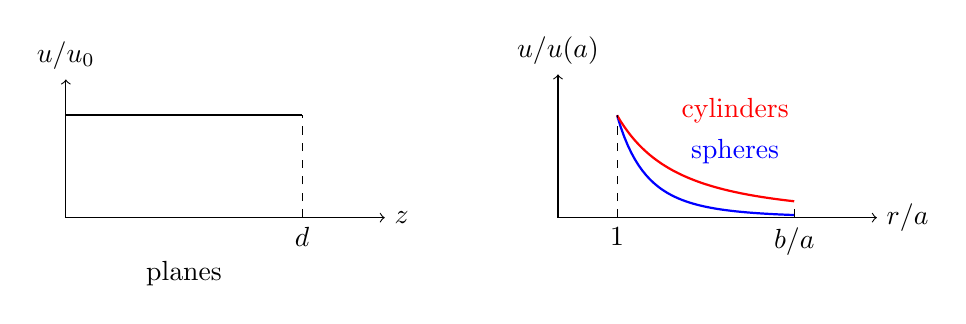
\begin{tikzpicture}[x=1.5cm,y=1.3cm]
\draw[->] (0,0)--(2.7,0) node[right] {$z$};
\draw[->] (0,0)--(0,1.35) node[above] {$u/u_0$};
\draw[thick] (0,1)--(2,1);
\draw[dashed] (2,0)--(2,1);
\node[below] at (2,0) {$d$};
\node at (1,-.55) {planes};
\begin{scope}[xshift=5.5cm]
\draw[->] (.5,0)--(3.2,0) node[right] {$r/a$};
\draw[->] (.5,0)--(.5,1.4) node[above] {$u/u(a)$};
\draw[blue,thick,domain=1:2.5,samples=50] plot (\x,{1/\x^4});
\draw[red,thick,domain=1:2.5,samples=50] plot (\x,{1/\x^2});
\draw[dashed] (1,0)--(1,1);
\draw[dashed] (2.5,0)--(2.5,.16);
\node[below] at (1,0) {$1$};
\node[below] at (2.5,0) {$b/a$};
\node[blue] at (2,.65) {spheres};
\node[red] at (2,1.05) {cylinders};
\end{scope}
\end{tikzpicture}
\end{center}


\Needspace{5\baselineskip}
\par\bigskip
\noindent\textbf{1.9}\quad Calculate the attractive force between conductors in the parallel plate capacitor (Problem 1.6a) and the parallel cylinder capacitor (Problem 1.7) for
\begin{enumerate}
\item[(a)] fixed charges on each conductor;
\item[(b)] fixed potential difference between conductors.
\end{enumerate}
\solution
Let positive force mean increasing separation $d$. For fixed charge,
$F_d=-\partial_d U$. For fixed voltage the source also exchanges energy:
$dW_{\rm source}=V\,dQ=V^2dC$. Since
$dU_{\rm field}=\tfrac12V^2dC$, the mechanical work is
$F_d\,dd=dW_{\rm source}-dU_{\rm field}=\tfrac12V^2dC$.
Equivalently, differentiate $U_{\rm field}-VQ=-\tfrac12CV^2$.
\begin{enumerate}
\item[(a)] For the planes, $U=Q^2d/(2\epsilon_0A)$, so
\[
\boxed{F_d=-\frac{Q^2}{2\epsilon_0A}.}
\]
For the wires use energy per length
$U'=\lambda^2\ln(d/a)/(2\pi\epsilon_0)$, obtaining
\[
\boxed{\frac{F_d}{L}=-\frac{\lambda^2}{2\pi\epsilon_0d}.}
\]
\item[(b)] With $C=\epsilon_0A/d$ for the planes,
\[
\boxed{F_d=\tfrac12V^2\frac{dC}{dd}
=-\frac{\epsilon_0AV^2}{2d^2}.}
\]
For the wires,
\[
\frac{dC'}{dd}=-\frac{\pi\epsilon_0}{d\ln^2(d/a)},\qquad
\boxed{\frac{F_d}{L}=-\frac{\pi\epsilon_0V^2}{2d\ln^2(d/a)}.}
\]
Substitution of $Q=CV$ or $\lambda=C'V$ recovers the fixed-charge formulas
at the same instantaneous state. All signs are negative, hence attractive.
\end{enumerate}


\Needspace{5\baselineskip}
\par\bigskip
\noindent\textbf{1.10}\quad Prove the \emph{mean value theorem}: For charge-free space the value of the electrostatic potential at any point is equal to the average of the potential over the surface of \emph{any} sphere centered on that point.
\solution
Let $B_R$ be a ball wholly contained in a charge-free region, centered at
$\mathbf x_0$, and let
\[
M(R)=\frac1{4\pi}\int\Phi(\mathbf x_0+R\widehat{\mathbf r})d\Omega.
\]
Differentiating at fixed solid angle and using $da=R^2d\Omega$ gives
\[
M'(R)=\frac1{4\pi R^2}\oint_{\partial B_R}\partial_n\Phi\,da
=\frac1{4\pi R^2}\int_{B_R}\nabla^2\Phi\,d^3x=0.
\]
Thus $M$ is independent of radius. Continuity implies
$\lim_{R\to0}M(R)=\Phi(\mathbf x_0)$, proving
\[
\boxed{\Phi(\mathbf x_0)=\frac1{4\pi R^2}\oint_{\partial B_R}\Phi\,da.}
\]
The entire ball must be free of charge and singularities, not just its surface.


\Needspace{5\baselineskip}
\par\bigskip
\noindent\textbf{1.11}\quad Use Gauss's theorem to prove that at the surface of a curved charged conductor, the normal derivative of the electric field is given by
\[
\frac{1}{E}\frac{\partial E}{\partial n} = -\left(\frac{1}{R_{1}}+\frac{1}{R_{2}}\right)
\]
where $R_{1}$ and $R_{2}$ are the principal radii of curvature of the surface.
\solution
Choose a small patch of area $dA$ and a tube whose sides follow the outward
normals. At normal distance $dn$, its area is, to first order,
\[
dA(dn)=dA\left(1+\frac{dn}{R_1}\right)
                 \left(1+\frac{dn}{R_2}\right)
=dA\left[1+\left(\frac1{R_1}+\frac1{R_2}\right)dn\right]+O(dn^2).
\]
The signed principal radii are positive on a convex surface with the outward
normal convention. The field is normal at the conductor. On the side faces the tangential field starts from zero and is $O(dn)$,
while their area is $O(dn)$. Side flux is therefore of
second order in the tube height, so the first-order charge-free flux balance is
\[
[E+\partial_nE\,dn]\,dA(dn)-E\,dA=0+O(dn^2).
\]
Expanding, dividing by $dA\,dn$, and taking the limit gives
\[
\partial_nE+E\left(\frac1{R_1}+\frac1{R_2}\right)=0,
\qquad
\boxed{\frac{\partial_nE}{E}=-\left(\frac1{R_1}+\frac1{R_2}\right).}
\]
The divided form applies where $E\ne0$; the undivided equation remains valid
where it vanishes. A sphere has $E\propto r^{-2}$ and gives $-2/R$; a
cylinder has $E\propto r^{-1}$ and gives $-1/R$, checking both curvature terms.


\Needspace{5\baselineskip}
\par\bigskip
\noindent\textbf{1.12}\quad Prove \emph{Green's reciprocation theorem}: If $\Phi$ is the potential due to a volume-charge density $\rho$ within a volume $V$ and a surface-charge density $\sigma$ on the conducting surface $S$ bounding the volume $V$, while $\Phi'$ is the potential due to another charge distribution $\rho'$ and $\sigma'$, then
\[
\int_{V}\rho\Phi'\;d^{3}x + \int_{S}\sigma\Phi'\;da = \int_{V}\rho'\Phi\;d^{3}x + \int_{S}\sigma'\Phi\;da
\]
\solution
Use the normal $\mathbf n$ pointing out of the field volume and into each
conductor. Since the electric field in the metal is zero, the conductor's
surface charge is $\sigma=\epsilon_0\partial_n\Phi$, and similarly for primes.
Green's second identity gives
\[
\int_V(\Phi\nabla^2\Phi'-\Phi'\nabla^2\Phi)d^3x
=\oint_S(\Phi\partial_n\Phi'-\Phi'\partial_n\Phi)da.
\]
Insert $\nabla^2\Phi=-\rho/\epsilon_0$ and its primed counterpart:
\[
\int_V(\rho\Phi'-\rho'\Phi)d^3x
=\oint_S(\sigma'\Phi-\sigma\Phi')da.
\]
Moving the surface terms to the respective sides proves
\[
\boxed{\int_V\rho\Phi'd^3x+\oint_S\sigma\Phi'da
=\int_V\rho'\Phi d^3x+\oint_S\sigma'\Phi da.}
\]
If a boundary is at infinity, the identity assumes the usual decay that makes
its surface contribution vanish; otherwise that boundary contribution must be retained.


\Needspace{5\baselineskip}
\par\bigskip
\noindent\textbf{1.13}\quad Two infinite grounded parallel conducting planes are separated by a distance $d$. A point charge $q$ is placed between the planes. Use the reciprocation theorem of Green to prove that the total induced charge on one of the planes is equal to $(-q)$ times the fractional perpendicular distance of the point charge from the other plane. (\emph{Hint}: As your comparison electrostatic problem with the same surfaces choose one whose charge densities and potential are known and simple.)
\solution
Take the planes at $z=0$ and $z=d$, and put $q$ at $z=z_0$.
The actual plane potentials are zero. For the comparison problem hold the
lower plane at $V_*$ and the upper at zero, without volume charge. Its potential is
\[
\Phi'(z)=V_*(1-z/d),\qquad\rho'=0.
\]
In the reciprocity relation all right-hand terms vanish, because the actual
potential on either conductor is zero. The left side is
\[
qV_*\left(1-\frac{z_0}{d}\right)+V_*Q_0=0.
\]
Dividing by $V_*$ gives
$\boxed{Q_0=-q(d-z_0)/d}$.
Interchanging the reference potentials similarly gives
$\boxed{Q_d=-qz_0/d}$. Their sum is $-q$, as also required by the Gaussian
surface enclosing the charge and both induced distributions.


\Needspace{5\baselineskip}
\par\bigskip
\noindent\textbf{1.14}\quad Consider the electrostatic Green functions of Section 1.10 for Dirichlet and Neumann boundary conditions on the surface $S$ bounding the volume $V$. Apply Green's theorem (1.35) with integration variable $\mathbf{y}$ and $\phi=G(\mathbf{x},\mathbf{y})$, $\psi=G(\mathbf{x}',\mathbf{y})$, with $\nabla^{2}_{y}G(\mathbf{z},\mathbf{y})=-4\pi\delta(\mathbf{y}-\mathbf{z})$. Find an expression for the difference $[G(\mathbf{x},\mathbf{x}')-G(\mathbf{x}',\mathbf{x})]$ in terms of an integral over the boundary surface $S$.
\begin{enumerate}
\item[(a)] For Dirichlet boundary conditions on the potential and the associated boundary condition on the Green function, show that $G_{D}(\mathbf{x},\mathbf{x}'\erratum{)}$ must be symmetric in $\mathbf{x}$ and $\mathbf{x}'$.
\item[(b)] For Neumann boundary conditions, use the boundary condition (1.45) for $G_{N}(\mathbf{x},\mathbf{x}')$ to show that $G_{N}(\mathbf{x},\mathbf{x}')$ is not symmetric in general, but that $G_{N}(\mathbf{x},\mathbf{x}')-F(\mathbf{x})$ is symmetric in $\mathbf{x}$ and $\mathbf{x}'$, where
\[
F(\mathbf{x}) = \frac{1}{S}\oint_{S}G_{N}(\mathbf{x},\mathbf{y})\;da_{y}
\]
\item[(c)] Show that the addition of $F(\mathbf{x})$ to the Green function does not affect the potential $\Phi(\mathbf{x})$. See problem 3.26 for an example of the Neumann Green function.
\end{enumerate}
\solution
Set $g(\mathbf y)=G(\mathbf x,\mathbf y)$ and
$h(\mathbf y)=G(\mathbf x',\mathbf y)$. Green's identity yields
\[
\begin{split}
\oint_S(g\partial_nh-h\partial_ng)da
&=\int_V(g\nabla_y^2h-h\nabla_y^2g)d^3y\\
&=-4\pi G(\mathbf x,\mathbf x')+4\pi G(\mathbf x',\mathbf x).
\end{split}
\]
Thus
\[
\boxed{G(\mathbf x,\mathbf x')-G(\mathbf x',\mathbf x)
=\frac1{4\pi}\oint_S(h\partial_ng-g\partial_nh)da.}
\]
\begin{enumerate}
\item[(a)] For $G_D$, both $g$ and $h$ vanish on $S$; the integral is zero.
\item[(b)] Jackson's normalization is
$\partial_{n_y}G_N(\mathbf z,\mathbf y)=-4\pi/S$. Substitution gives
\[
G_N(\mathbf x,\mathbf x')-G_N(\mathbf x',\mathbf x)
=\frac1S\oint_S[g(\mathbf y)-h(\mathbf y)]da
=F(\mathbf x)-F(\mathbf x').
\]
Rearrangement shows that $G_N(\mathbf x,\mathbf x')-F(\mathbf x)$ is symmetric.
\item[(c)] The Neumann potential formula is
\[
\Phi(\mathbf x)=\langle\Phi\rangle_S+
\frac1{4\pi\epsilon_0}\int_V\rho(\mathbf y)G_N(\mathbf x,\mathbf y)d^3y
+\frac1{4\pi}\oint_SG_N(\mathbf x,\mathbf y)\partial_n\Phi(\mathbf y)da.
\]
Adding any function $f(\mathbf x)$ independent of $\mathbf y$ changes this by
\[
\Delta\Phi=\frac{f(\mathbf x)}{4\pi}
\left[\frac1{\epsilon_0}\int_V\rho\,d^3y+\oint_S\partial_n\Phi\,da\right]=0,
\]
because the divergence theorem and Poisson's equation give
$\oint\partial_n\Phi=\int\nabla^2\Phi=-\int\rho/\epsilon_0$.
This applies to adding $F$ as asked, or subtracting it to obtain the symmetric
kernel. The independent additive constant $\langle\Phi\rangle_S$ still fixes
the potential's gauge.
\end{enumerate}


\Needspace{5\baselineskip}
\par\bigskip
\noindent\textbf{1.15}\quad Prove \emph{Thomson's theorem}: If a number of surfaces are fixed in position and a given total charge is placed on each surface, then the electrostatic energy in the region bounded by the surfaces is an absolute minimum when the charges are placed so that every surface is an equipotential, as happens when they are conductors.
\solution
Let $\rho_0$ (including surface charges) be the equipotential distribution,
with field $\mathbf E_0$ and potential $\Phi_0$. Any other admissible
redistribution is $\rho_0+\delta\rho$, with field
$\mathbf E_0+\delta\mathbf E$, and with $\delta Q_i=0$ on each surface.
Expanding the field energy gives
\[
U-U_0=\epsilon_0\int\mathbf E_0\cdot\delta\mathbf E\,d^3x
+\frac{\epsilon_0}{2}\int|\delta\mathbf E|^2d^3x.
\]
Integrating the cross term by parts over all field space, or treating surface
charges as distributions, yields
\[
\epsilon_0\int\nabla\Phi_0\cdot\nabla\delta\Phi\,d^3x
=\int\Phi_0\delta\rho\,d^3x
=\sum_i\Phi_{0i}\delta Q_i=0.
\]
Consequently
\[
\boxed{U-U_0=\frac{\epsilon_0}{2}\int|\delta\mathbf E|^2d^3x\ge0.}
\]
This is a global minimum, not just a stationary value. Equality requires no
change of field. Fixed additional volume charges, if present, are left
unchanged in the variation.


\Needspace{5\baselineskip}
\par\bigskip
\noindent\textbf{1.16}\quad Prove the following theorem: If a number of conducting surfaces are fixed in position with a given total charge on each, the introduction of an uncharged, insulated conductor into the region bounded by the surfaces \erratum{cannot increase} the electrostatic energy. \erratum{The decrease is strict if the field changes.}
\solution
Before inserting the new conductor, denote the equilibrium energy by $U_0$.
In the enlarged set of possible charge distributions, consider the trial
configuration that retains every old charge and places zero excess charge
everywhere on the new conductor. It has the prescribed old charges and zero
total new charge, so it is an admissible charge distribution for Thomson's
minimization problem, although it is generally not an equilibrium distribution.
Its field and energy, integrated also through the new body's volume, are the
old ones: $U_{\rm trial}=U_0$.

The new equilibrium minimizes the energy over this enlarged set. Therefore
\[
\boxed{U_{\rm new}\le U_{\rm trial}=U_0.}
\]
More explicitly, applying the proof of Problem 1.15 with the new equilibrium
as the reference gives
\[
U_0-U_{\rm new}=\frac{\epsilon_0}{2}
\int|\mathbf E_0-\mathbf E_{\rm new}|^2d^3x\ge0.
\]
The inequality is strict if insertion changes the field. Equality is possible
when the inserted body occupies a region that was already field-free.
The old conductors are insulated with fixed charges; maintaining fixed
potentials would involve additional work by voltage sources.


\Needspace{5\baselineskip}
\par\bigskip
\noindent\textbf{1.17}\quad A volume $V$ in vacuum is bounded by a surface $S$ consisting of several separate conducting surfaces $S_{i}$. One conductor is held at \emph{unit} potential and all the other conductors at zero potential.
\begin{enumerate}
\item[(a)] Show that the capacitance of the one conductor is given by
\[
C = \epsilon_{0}\int_{V}|\nabla\Phi|^{2}\;d^{3}x
\]
where $\Phi(\mathbf{x})$ is the solution for the potential.
\item[(b)] Show that the true capacitance $C$ is always less than or equal to the quantity
\[
C[\Psi] = \epsilon_{0}\int_{V}|\nabla\Psi|^{2}\;d^{3}x
\]
where $\Psi$ is any trial function satisfying the boundary conditions on the conductors. This is a variational principle for the capacitance that yields an \emph{upper bound}.
\end{enumerate}
\solution
\begin{enumerate}
\item[(a)] There is no volume charge. With the normal directed out of $V$,
Green's first identity gives
\[
\int_V|\nabla\Phi|^2d^3x
=\oint_S\Phi\partial_n\Phi\,da
=\int_{S_1}\partial_n\Phi\,da=Q_1/\epsilon_0.
\]
Only $S_1$ contributes, because its potential is one and all others are zero.
Since $Q_1=C\times1$, this proves
$\boxed{C=\epsilon_0\int_V|\nabla\Phi|^2d^3x}$.
\item[(b)] Write a trial function as $\Psi=\Phi+\eta$ with $\eta=0$ on every
conductor. Then
\[
C[\Psi]-C
=2\epsilon_0\int_V\nabla\Phi\cdot\nabla\eta\,d^3x
+\epsilon_0\int_V|\nabla\eta|^2d^3x.
\]
The first integral is
$\oint\eta\partial_n\Phi\,da-\int\eta\nabla^2\Phi\,d^3x=0$.
Thus
\[
\boxed{C[\Psi]-C=\epsilon_0\int_V|\nabla\eta|^2d^3x\ge0.}
\]
Trial functions need finite field energy and the specified boundary values;
they need not solve Laplace's equation.
\end{enumerate}


\Needspace{5\baselineskip}
\par\bigskip
\noindent\textbf{1.18}\quad Consider the configuration of conductors of Problem 1.17, with all conductors except $S_{1}$ held at zero potential.
\begin{enumerate}
\item[(a)] Show that the potential $\Phi(\mathbf{x})$ anywhere in the volume $V$ \emph{and} on any of the surfaces $S_{i}$ can be written
\[
\Phi(\mathbf{x}) = \frac{1}{4\pi\epsilon_{0}}\oint_{S_{1}}\sigma_{1}(\mathbf{x}')G(\mathbf{x},\mathbf{x}')\;da'
\]
where $\sigma_{1}(\mathbf{x}')$ is the surface charge density on $S_{1}$ and $G(\mathbf{x},\mathbf{x}')$ is the Green function potential for a point charge in the presence of all the surfaces that are held at zero potential (but with $S_{1}$ absent). Show also that the electrostatic energy is
\[
W = \frac{1}{8\pi\epsilon_{0}}\oint_{S_{1}}da\oint_{S_{1}}da'\;\sigma_{1}(\mathbf{x})G(\mathbf{x},\mathbf{x}')\sigma_{1}(\mathbf{x}')
\]
where the integrals are only over the surface $S_{1}$.
\item[(b)] Show that the variational expression
\[
C^{-1}[\sigma] = \frac{\displaystyle\oint_{S_{1}}da\oint_{S_{1}}da'\;\sigma(\mathbf{x})G(\mathbf{x},\mathbf{x}')\sigma(\mathbf{x}')}{4\pi\epsilon_{0}\left[\displaystyle\oint_{S_{1}}\sigma(\mathbf{x})\;da\right]^{2}}
\]
with an arbitrary integrable function $\sigma(\mathbf{x})$ defined on $S_{1}$, \erratum{having nonzero total charge and finite electrostatic energy}, is stationary for small variations of $\sigma$ away from $\sigma_{1}$. Use Thomson's theorem to prove that the reciprocal of $C^{-1}[\sigma]$ gives a \emph{lower bound} to the true capacitance of the conductor $S_{1}$.
\end{enumerate}
\solution
\begin{enumerate}
\item[(a)] Remove $S_1$ and use the Dirichlet Green function for the remaining
grounded conductors. An element $dq=\sigma_1(\mathbf x')da'$ produces
$d\Phi=G(\mathbf x,\mathbf x')dq/(4\pi\epsilon_0)$, including the response
of those grounded conductors. Superposition gives
\[
\boxed{\Phi(\mathbf x)=\frac1{4\pi\epsilon_0}
\oint_{S_1}\sigma_1(\mathbf x')G(\mathbf x,\mathbf x')da'.}
\]
This is also the continuous single-layer potential at the surface itself.
The electrostatic energy is $W=\tfrac12\sum_i\int_{S_i}\sigma_i\Phi_i\,da$.
All grounded surfaces have $\Phi_i=0$, so substitution leaves
\[
\boxed{W=\frac1{8\pi\epsilon_0}\oint_{S_1}\!da\oint_{S_1}\!da'\,
\sigma_1(\mathbf x)G(\mathbf x,\mathbf x')\sigma_1(\mathbf x').}
\]
\item[(b)] Write $Q[\sigma]=\int\sigma da$ and
$B[\sigma]=\iint\sigma G\sigma\,da\,da'$. Then
$C^{-1}[\sigma]=B/(4\pi\epsilon_0Q^2)=2W[\sigma]/Q^2$.
Symmetry of $G$ gives
\[
\delta B=2\int\delta\sigma(\mathbf x)
\left[\int G(\mathbf x,\mathbf x')\sigma_1(\mathbf x')da'\right]da
=8\pi\epsilon_0V_1\delta Q.
\]
At equilibrium $B=4\pi\epsilon_0V_1Q$, and hence
\[
\delta C^{-1}=\frac{\delta B}{4\pi\epsilon_0Q^2}
-\frac{2B\delta Q}{4\pi\epsilon_0Q^3}=0.
\]
Because this quotient is unchanged by rescaling $\sigma$, compare trial
functions at the same nonzero charge $Q$. If $\delta\sigma=\sigma-\sigma_1$
and $\int\delta\sigma=0$, the energy cross term is
$V_1\int\delta\sigma=0$. The remaining term is
\[
W[\sigma]-W[\sigma_1]=\frac1{8\pi\epsilon_0}\iint\delta\sigma G\delta\sigma
=\frac{\epsilon_0}{2}\int|\nabla\delta\Phi|^2d^3x\ge0.
\]
Thus $C^{-1}[\sigma]\ge C^{-1}$ and
$\boxed{1/C^{-1}[\sigma]\le C}$.
The admissible trial density must have nonzero total charge and finite
self-energy; integrability alone does not guarantee the latter. An infinite
energy trial supplies only the trivial zero lower bound.
\end{enumerate}


\Needspace{5\baselineskip}
\par\bigskip
\noindent\textbf{1.19}\quad For the cylindrical capacitor of Problem 1.6c, evaluate the variational upper bound of Problem 1.17b with the naive trial function, $\Psi_{1}(\rho)=(b-\rho)/(b-a)$. Compare the variational result with the exact result for $b/a=1.5$, 2, 3. Explain the trend of your results in terms of the functional form of $\Psi_{1}$. An improved trial function is treated by \emph{Collin} (pp.~275--277).
\solution
In the long-cylinder approximation,
$\nabla\Psi_1=-\widehat{\boldsymbol\rho}/(b-a)$, so
\[
C[\Psi_1]=\epsilon_0L\int_a^b\frac{2\pi\rho\,d\rho}{(b-a)^2}
=\pi\epsilon_0L\frac{b+a}{b-a}.
\]
Divide by $C=2\pi\epsilon_0L/\ln(b/a)$ and set $t=b/a$:
\[
\boxed{\frac{C[\Psi_1]}C=\frac{t+1}{2(t-1)}\ln t.}
\]
The ratios at $t=1.5,2,3$ are $1.013663$, $1.039721$, and $1.098612$,
i.e. upper-bound errors of $1.37\%$, $3.97\%$, and $9.86\%$.
The exact potential is $\Phi=\ln(b/\rho)/\ln(b/a)$, whose gradient varies
as $1/\rho$. A constant-gradient linear trial is close when the gap is narrow
but cannot reproduce that variation across a wide annulus. In particular,
putting $t=1+\delta$ gives
\[
\frac{2+\delta}{2\delta}
\left(\delta-\frac{\delta^2}{2}+\frac{\delta^3}{3}-\cdots\right)
=1+\frac{\delta^2}{12}+O(\delta^3),
\]
which verifies approach to the exact result as the gap shrinks.


\Needspace{5\baselineskip}
\par\bigskip
\noindent\textbf{1.20}\quad In estimating the capacitance of a given configuration of conductors, comparison with known capacitances is often helpful. Consider two configurations of $n$ conductors in which the $(n-1)$ conductors held at zero potential are the same, but the one conductor whose capacitance we wish to know is different. In particular, let the conductor in one configuration have a closed surface $S_{1}$ and in the other configuration have surface $S_{1}'$, with $S_{1}'$ totally inside $S_{1}$.
\begin{enumerate}
\item[(a)] Use the extremum principle of Section 1.12 and the variational principle of Problem 1.17 to prove that the capacitance $C'$ of the conductor with surface $S_{1}'$ is less than or equal to the capacitance $C$ of the conductor with surface $S_{1}$ that encloses $S_{1}'$.
\item[(b)] Set upper and lower limits for the capacitance of a conducting cube of side $a$. Compare your limits and also their average with the numerical value, $C\simeq0.655(4\pi\epsilon_{0}a)$.
\item[(c)] By how much do you estimate the capacitance per unit length of the two-wire system of Problem 1.7 will change (larger? smaller?) if \emph{one} of the wires is replaced by a wire of square cross section whose side is equal to its diameter?
\end{enumerate}
\solution
\begin{enumerate}
\item[(a)] Normalize the larger conductor to unit potential, and call its
exterior solution $\Phi$. For the smaller-conductor problem choose the trial
potential equal to $\Phi$ outside $S_1$ and equal to one throughout the
space between $S_1'$ and $S_1$. It is continuous and satisfies all the
smaller problem's Dirichlet data. Its gradient vanishes in the added region,
so its variational integral is exactly $C$. Problem 1.17 therefore gives
$\boxed{C'\le C}$.
\item[(b)] The cube contains a sphere of radius $a/2$ and lies inside a sphere
of radius $\sqrt3a/2$. Using $C_{\rm sphere}=4\pi\epsilon_0R$ gives
\[
\boxed{\frac12\le\frac{C_{\rm cube}}{4\pi\epsilon_0a}\le\frac{\sqrt3}{2}
=0.866025.}
\]
The average of the bounds is $(1+\sqrt3)/4=0.683013$. Relative to the quoted
$0.655$, the lower bound is $23.66\%$ low, the upper $32.22\%$ high, and the
average $4.28\%$ high. The average is an estimate, not a variational bound.
\item[(c)] A square wire of side $2a_1$ contains the old round wire of radius
$a_1$ and is contained in a round wire of radius $\sqrt2a_1$.
The two-conductor capacitance is unchanged if the labels of the grounded and
unit-potential wires are exchanged, so part (a) applies to replacing this wire.
Writing $\ell=\ln[d/\sqrt{a_1a_2}]$, the thin-wire formula gives
\[
C'_0=\frac{\pi\epsilon_0}{\ell},\qquad
C'_0\le C'_{\rm square}\lesssim
\frac{\pi\epsilon_0}{\ell-\tfrac14\ln2}.
\]
Thus the capacitance increases, with estimated fractional increase between
zero and
\[
\frac{(\ln2)/4}{\ell-(\ln2)/4}.
\]
A simple midpoint estimate is half this interval. For the lines in 1.7,
$\ell=\pi\epsilon_0/(1.2\times10^{-11})\simeq2.318$; the interval is
$0$ to $8.08\%$ and its midpoint is about $4.04\%$.
The monotonicity is exact, while these numerical percentages inherit the
thin-wire approximation.
\end{enumerate}


\Needspace{5\baselineskip}
\par\bigskip
\noindent\textbf{1.21}\quad A two-dimensional potential problem consists of a unit square area ($0\leq x\leq1$, $0\leq y\leq1$) bounded by ``surfaces'' held at zero potential. Over the entire square there is a uniform charge density of unit strength (per unit length in $z$).
\begin{enumerate}
\item[(a)] Apply the variational principle (1.63) for the Poisson equation with the ``variational'' trial function $\Psi(x,y)=A\cdot x(1-x)\cdot y(1-y)$ to determine the best value of the constant $A$. [I use quotation marks around variational because there are no parameters to vary except the overall scale.]
\item[(b)] The exact (albeit series) solution for this problem is [see Problems 2.15 and 2.16]
\[
4\pi\epsilon_{0}\Phi(x,y) = \frac{16}{\pi^{2}}\sum_{m=0}^{\infty}\frac{\sin[(2m+1)\pi x]}{(2m+1)^{3}}\left\{1-\frac{\cosh[(2m+1)\pi(y-\frac{1}{2})]}{\cosh[(2m+1)\pi/2]}\right\}
\]
For $y=0.25$ and $y=0.5$, plot and compare the simple variational solution of part a with the exact solution as functions of $x$.
\end{enumerate}
\solution
\begin{enumerate}
\item[(a)] Put $f=x(1-x)y(1-y)$ and $\Psi=Af$. For unit charge density the
functional (1.63) is
\[
I[A]=\frac12 A^2\int_0^1\!\int_0^1|\nabla f|^2dxdy
-\frac{A}{\epsilon_0}\int_0^1\!\int_0^1f\,dxdy.
\]
The elementary integrals are
\[
\int_0^1x(1-x)dx=\frac16,\quad
\int_0^1x^2(1-x)^2dx=\frac1{30},\quad
\int_0^1(1-2x)^2dx=\frac13.
\]
Consequently $\int f=1/36$ and
$\int|\nabla f|^2=2(1/3)(1/30)=1/45$, giving
\[
I[A]=\frac{A^2}{90}-\frac{A}{36\epsilon_0},\qquad
I'[A]=\frac A{45}-\frac1{36\epsilon_0}=0.
\]
Thus $\boxed{A=5/(4\epsilon_0)}$, and $I''=1/45>0$.
In the book's plotted normalization,
\[\boxed{u_{\rm trial}=4\pi\epsilon_0\Psi=5\pi x(1-x)y(1-y).}\]
\item[(b)] Write $k_n=n\pi$ for positive odd $n$. The supplied exact series is
\[
u=\frac{16}{\pi^2}\sum_{n\ {\rm odd}>0}\frac{\sin k_nx}{n^3}
\left[1-\frac{\cosh(k_n(y-1/2))}{\cosh(k_n/2)}\right].
\]
The boundary factors vanish at $x=0,1$ and $y=0,1$. Applying the Laplacian
cancels the two derivatives of the hyperbolic term, leaving
\[
\nabla^2u=-16\sum_{n\ {\rm odd}>0}\frac{\sin(n\pi x)}n=-4\pi,
\]
where $1=(4/\pi)\sum_{n\ {\rm odd}>0}\sin(n\pi x)/n$ is the sine expansion
of a constant on $0<x<1$. Thus the normalization indeed corresponds to
$\rho=1$. The comparison is
\begin{center}
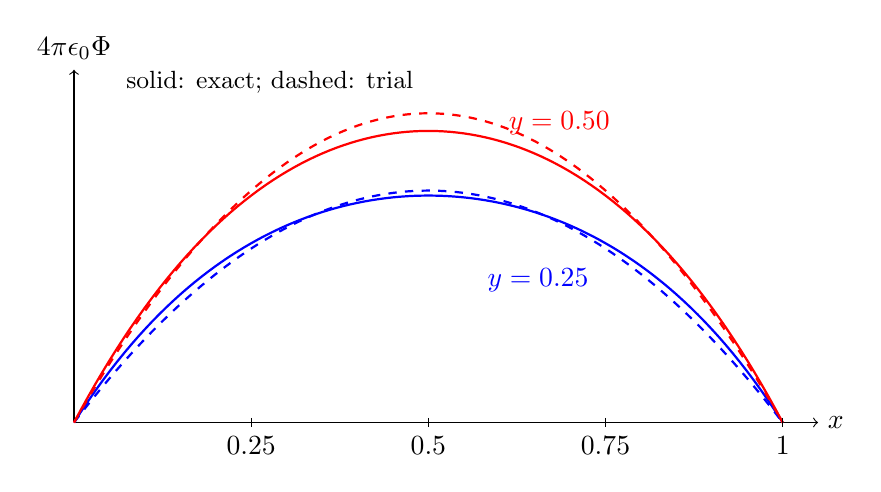
\begin{tikzpicture}[x=9cm,y=4cm]
\draw[->] (0,0)--(1.05,0) node[right] {$x$};
\draw[->] (0,0)--(0,1.12) node[above] {$4\pi\epsilon_0\Phi$};
\draw[blue,thick] plot coordinates {(0.000000,0.000000) (0.010000,0.034737) (0.020000,0.068250) (0.030000,0.100571) (0.040000,0.131732) (0.050000,0.161767) (0.060000,0.190705) (0.070000,0.218579) (0.080000,0.245418) (0.090000,0.271252) (0.100000,0.296111) (0.110000,0.320022) (0.120000,0.343014) (0.130000,0.365112) (0.140000,0.386343) (0.150000,0.406731) (0.160000,0.426300) (0.170000,0.445074) (0.180000,0.463074) (0.190000,0.480322) (0.200000,0.496837) (0.210000,0.512640) (0.220000,0.527749) (0.230000,0.542181) (0.240000,0.555954) (0.250000,0.569083) (0.260000,0.581583) (0.270000,0.593470) (0.280000,0.604756) (0.290000,0.615456) (0.300000,0.625580) (0.310000,0.635140) (0.320000,0.644148) (0.330000,0.652614) (0.340000,0.660546) (0.350000,0.667955) (0.360000,0.674848) (0.370000,0.681233) (0.380000,0.687117) (0.390000,0.692506) (0.400000,0.697408) (0.410000,0.701826) (0.420000,0.705766) (0.430000,0.709233) (0.440000,0.712230) (0.450000,0.714760) (0.460000,0.716826) (0.470000,0.718431) (0.480000,0.719576) (0.490000,0.720263) (0.500000,0.720492) (0.510000,0.720263) (0.520000,0.719576) (0.530000,0.718431) (0.540000,0.716826) (0.550000,0.714760) (0.560000,0.712230) (0.570000,0.709233) (0.580000,0.705766) (0.590000,0.701826) (0.600000,0.697408) (0.610000,0.692506) (0.620000,0.687117) (0.630000,0.681233) (0.640000,0.674848) (0.650000,0.667955) (0.660000,0.660546) (0.670000,0.652614) (0.680000,0.644148) (0.690000,0.635140) (0.700000,0.625580) (0.710000,0.615456) (0.720000,0.604756) (0.730000,0.593470) (0.740000,0.581583) (0.750000,0.569083) (0.760000,0.555954) (0.770000,0.542181) (0.780000,0.527749) (0.790000,0.512640) (0.800000,0.496837) (0.810000,0.480322) (0.820000,0.463074) (0.830000,0.445074) (0.840000,0.426300) (0.850000,0.406731) (0.860000,0.386343) (0.870000,0.365112) (0.880000,0.343014) (0.890000,0.320022) (0.900000,0.296111) (0.910000,0.271252) (0.920000,0.245418) (0.930000,0.218579) (0.940000,0.190705) (0.950000,0.161767) (0.960000,0.131732) (0.970000,0.100571) (0.980000,0.068250) (0.990000,0.034737) (1.000000,0.000000)};
\draw[blue,thick,dashed] plot coordinates {(0.000000,0.000000) (0.010000,0.029158) (0.020000,0.057727) (0.030000,0.085707) (0.040000,0.113097) (0.050000,0.139899) (0.060000,0.166112) (0.070000,0.191735) (0.080000,0.216770) (0.090000,0.241215) (0.100000,0.265072) (0.110000,0.288339) (0.120000,0.311018) (0.130000,0.333107) (0.140000,0.354607) (0.150000,0.375518) (0.160000,0.395841) (0.170000,0.415574) (0.180000,0.434718) (0.190000,0.453273) (0.200000,0.471239) (0.210000,0.488616) (0.220000,0.505404) (0.230000,0.521603) (0.240000,0.537212) (0.250000,0.552233) (0.260000,0.566665) (0.270000,0.580507) (0.280000,0.593761) (0.290000,0.606426) (0.300000,0.618501) (0.310000,0.629988) (0.320000,0.640885) (0.330000,0.651193) (0.340000,0.660913) (0.350000,0.670043) (0.360000,0.678584) (0.370000,0.686536) (0.380000,0.693899) (0.390000,0.700673) (0.400000,0.706858) (0.410000,0.712454) (0.420000,0.717461) (0.430000,0.721879) (0.440000,0.725708) (0.450000,0.728948) (0.460000,0.731598) (0.470000,0.733660) (0.480000,0.735133) (0.490000,0.736016) (0.500000,0.736311) (0.510000,0.736016) (0.520000,0.735133) (0.530000,0.733660) (0.540000,0.731598) (0.550000,0.728948) (0.560000,0.725708) (0.570000,0.721879) (0.580000,0.717461) (0.590000,0.712454) (0.600000,0.706858) (0.610000,0.700673) (0.620000,0.693899) (0.630000,0.686536) (0.640000,0.678584) (0.650000,0.670043) (0.660000,0.660913) (0.670000,0.651193) (0.680000,0.640885) (0.690000,0.629988) (0.700000,0.618501) (0.710000,0.606426) (0.720000,0.593761) (0.730000,0.580507) (0.740000,0.566665) (0.750000,0.552233) (0.760000,0.537212) (0.770000,0.521603) (0.780000,0.505404) (0.790000,0.488616) (0.800000,0.471239) (0.810000,0.453273) (0.820000,0.434718) (0.830000,0.415574) (0.840000,0.395841) (0.850000,0.375518) (0.860000,0.354607) (0.870000,0.333107) (0.880000,0.311018) (0.890000,0.288339) (0.900000,0.265072) (0.910000,0.241215) (0.920000,0.216770) (0.930000,0.191735) (0.940000,0.166112) (0.950000,0.139899) (0.960000,0.113097) (0.970000,0.085707) (0.980000,0.057727) (0.990000,0.029158) (1.000000,0.000000)};
\draw[red,thick] plot coordinates {(0.000000,0.000000) (0.010000,0.041806) (0.020000,0.082377) (0.030000,0.121733) (0.040000,0.159895) (0.050000,0.196885) (0.060000,0.232721) (0.070000,0.267426) (0.080000,0.301020) (0.090000,0.333522) (0.100000,0.364953) (0.110000,0.395332) (0.120000,0.424679) (0.130000,0.453014) (0.140000,0.480354) (0.150000,0.506718) (0.160000,0.532125) (0.170000,0.556592) (0.180000,0.580136) (0.190000,0.602775) (0.200000,0.624526) (0.210000,0.645403) (0.220000,0.665423) (0.230000,0.684602) (0.240000,0.702953) (0.250000,0.720492) (0.260000,0.737231) (0.270000,0.753184) (0.280000,0.768364) (0.290000,0.782783) (0.300000,0.796453) (0.310000,0.809385) (0.320000,0.821589) (0.330000,0.833076) (0.340000,0.843855) (0.350000,0.853936) (0.360000,0.863326) (0.370000,0.872034) (0.380000,0.880067) (0.390000,0.887433) (0.400000,0.894136) (0.410000,0.900184) (0.420000,0.905581) (0.430000,0.910333) (0.440000,0.914442) (0.450000,0.917913) (0.460000,0.920749) (0.470000,0.922952) (0.480000,0.924525) (0.490000,0.925467) (0.500000,0.925782) (0.510000,0.925467) (0.520000,0.924525) (0.530000,0.922952) (0.540000,0.920749) (0.550000,0.917913) (0.560000,0.914442) (0.570000,0.910333) (0.580000,0.905581) (0.590000,0.900184) (0.600000,0.894136) (0.610000,0.887433) (0.620000,0.880067) (0.630000,0.872034) (0.640000,0.863326) (0.650000,0.853936) (0.660000,0.843855) (0.670000,0.833076) (0.680000,0.821589) (0.690000,0.809385) (0.700000,0.796453) (0.710000,0.782783) (0.720000,0.768364) (0.730000,0.753184) (0.740000,0.737231) (0.750000,0.720492) (0.760000,0.702953) (0.770000,0.684602) (0.780000,0.665423) (0.790000,0.645403) (0.800000,0.624526) (0.810000,0.602775) (0.820000,0.580136) (0.830000,0.556592) (0.840000,0.532125) (0.850000,0.506718) (0.860000,0.480354) (0.870000,0.453014) (0.880000,0.424679) (0.890000,0.395332) (0.900000,0.364953) (0.910000,0.333522) (0.920000,0.301020) (0.930000,0.267426) (0.940000,0.232721) (0.950000,0.196885) (0.960000,0.159895) (0.970000,0.121733) (0.980000,0.082377) (0.990000,0.041806) (1.000000,0.000000)};
\draw[red,thick,dashed] plot coordinates {(0.000000,0.000000) (0.010000,0.038877) (0.020000,0.076969) (0.030000,0.114275) (0.040000,0.150796) (0.050000,0.186532) (0.060000,0.221482) (0.070000,0.255647) (0.080000,0.289027) (0.090000,0.321621) (0.100000,0.353429) (0.110000,0.384452) (0.120000,0.414690) (0.130000,0.444143) (0.140000,0.472810) (0.150000,0.500691) (0.160000,0.527788) (0.170000,0.554098) (0.180000,0.579624) (0.190000,0.604364) (0.200000,0.628319) (0.210000,0.651488) (0.220000,0.673872) (0.230000,0.695470) (0.240000,0.716283) (0.250000,0.736311) (0.260000,0.755553) (0.270000,0.774010) (0.280000,0.791681) (0.290000,0.808567) (0.300000,0.824668) (0.310000,0.839983) (0.320000,0.854513) (0.330000,0.868258) (0.340000,0.881217) (0.350000,0.893390) (0.360000,0.904779) (0.370000,0.915382) (0.380000,0.925199) (0.390000,0.934231) (0.400000,0.942478) (0.410000,0.949939) (0.420000,0.956615) (0.430000,0.962505) (0.440000,0.967611) (0.450000,0.971930) (0.460000,0.975465) (0.470000,0.978213) (0.480000,0.980177) (0.490000,0.981355) (0.500000,0.981748) (0.510000,0.981355) (0.520000,0.980177) (0.530000,0.978213) (0.540000,0.975465) (0.550000,0.971930) (0.560000,0.967611) (0.570000,0.962505) (0.580000,0.956615) (0.590000,0.949939) (0.600000,0.942478) (0.610000,0.934231) (0.620000,0.925199) (0.630000,0.915382) (0.640000,0.904779) (0.650000,0.893390) (0.660000,0.881217) (0.670000,0.868258) (0.680000,0.854513) (0.690000,0.839983) (0.700000,0.824668) (0.710000,0.808567) (0.720000,0.791681) (0.730000,0.774010) (0.740000,0.755553) (0.750000,0.736311) (0.760000,0.716283) (0.770000,0.695470) (0.780000,0.673872) (0.790000,0.651488) (0.800000,0.628319) (0.810000,0.604364) (0.820000,0.579624) (0.830000,0.554098) (0.840000,0.527788) (0.850000,0.500691) (0.860000,0.472810) (0.870000,0.444143) (0.880000,0.414690) (0.890000,0.384452) (0.900000,0.353429) (0.910000,0.321621) (0.920000,0.289027) (0.930000,0.255647) (0.940000,0.221482) (0.950000,0.186532) (0.960000,0.150796) (0.970000,0.114275) (0.980000,0.076969) (0.990000,0.038877) (1.000000,0.000000)};
\node[blue,anchor=west] at (.57,.45) {$y=0.25$};
\node[red,anchor=west] at (.60,.95) {$y=0.50$};
\node[anchor=west,font=\small] at (.06,1.08) {solid: exact; dashed: trial};
\foreach \x in {0.25,0.5,0.75,1} \draw (\x,.015)--(\x,-.015) node[below] {$\x$};
\end{tikzpicture}

\end{center}
At $(1/2,1/4)$ the exact and trial values are $0.720492$ and
$15\pi/64=0.736311$; at the center they are $0.925782$ and
$5\pi/16=0.981748$. The respective errors are about $2.20\%$ and $6.04\%$.
The variational principle minimizes the functional, not the pointwise error,
so it does not make this potential a pointwise upper bound everywhere.
The numerical series uses the stable ratio
\[
\frac{\cosh(k(y-1/2))}{\cosh(k/2)}
=\frac{e^{-ky}+e^{-k(1-y)}}{1+e^{-k}},
\]
which avoids overflow for large $k$.
\end{enumerate}


\Needspace{5\baselineskip}
\par\bigskip
\noindent\textbf{1.22}\quad Two-dimensional relaxation calculations commonly use sites on a square lattice with spacing $\Delta x=\Delta y=h$, and label the sites by $(i,j)$, where $i,j$ are integers and $x_{i}=ih+x_{0}$, $y_{j}=jh+y_{0}$. The value of the potential at $(i,j)$ can be approximated by the average of the values at neighboring sites. [Recall the relevant theorem about harmonic functions.] But what average?
\begin{enumerate}
\item[(a)] If $F(x,y)$ is a well-behaved function in the neighborhood of the origin, but not necessarily harmonic, by explicit Taylor series expansions, show that the ``cross'' sum
\[
S_{\mathrm{c}} = F(h,0)+F(0,h)+F(-h,0)+F(0,-h)
\]
can be expressed as
\[
S_{\mathrm{c}} = 4F(0,0)+h^{2}\nabla^{2}F+\frac{h^{4}}{12}\left(F_{xxxx}+F_{yyyy}\right)+O(h^{6})
\]
\item[(b)] Similarly, show that the ``square'' sum,
\[
S_{\mathrm{s}} = F(h,h)+F(-h,h)+F(-h,-h)+F(h,-h)
\]
can be expressed as
\[
S_{\mathrm{s}} = 4F(0,0)+2h^{2}\nabla^{2}F-\frac{h^{4}}{3}\left(F_{xxxx}+F_{yyyy}\right)+\frac{h^{4}}{2}\nabla^{2}(\nabla^{2}F)+O(h^{6})
\]
Here $F_{xxxx}$ is the fourth partial derivative of $F$ with respect to $x$, evaluated at $x=0$, $y=0$, etc. If $\nabla^{2}F=0$, the averages $S_{\mathrm{c}}/4$ and $S_{\mathrm{s}}/4$ each give the value of $F(0,0)$, correct to order $h^{3}$ inclusive. Note that an improvement can be obtained by forming the ``improved'' average,
\[
\langle\!\langle F(0,0)\rangle\!\rangle = \frac{1}{5}\left[S_{\mathrm{c}}+\frac{1}{4}S_{\mathrm{s}}\right]
\]
where
\[
\langle\!\langle F(0,0)\rangle\!\rangle = F(0,0)+\frac{3}{10}h^{2}\nabla^{2}F+\frac{h^{4}}{40}\nabla^{2}(\nabla^{2}F)+O(h^{6})
\]
If $\nabla^{2}F=0$, then \erratum{the improved average} gives $F(0,0)$, correct to order $h^{5}$ inclusive. For Poisson's equation, the charge density and its lowest order Laplacian can be inserted for the same accuracy.
\end{enumerate}
\solution
Write all derivatives below at the origin. The multivariate Taylor series is
\[
F(x,y)=\sum_{p+q\le5}\frac{x^py^q}{p!q!}\partial_x^p\partial_y^qF
+O((|x|+|y|)^6).
\]
\begin{enumerate}
\item[(a)] Pairing opposite points cancels odd powers:
\[
F(h,0)+F(-h,0)=2F+h^2F_{xx}+\frac{h^4}{12}F_{xxxx}+O(h^6).
\]
The analogous $y$ pair gives
\[
\boxed{S_c=4F+h^2\nabla^2F+\frac{h^4}{12}(F_{xxxx}+F_{yyyy})+O(h^6).}
\]
\item[(b)] In the four diagonal points, terms with either odd $p$ or odd $q$
cancel. The surviving terms through degree four are
\[
S_s=4F+2h^2(F_{xx}+F_{yy})
+\frac{h^4}{6}(F_{xxxx}+F_{yyyy})+h^4F_{xxyy}+O(h^6).
\]
Since $\nabla^4F=F_{xxxx}+2F_{xxyy}+F_{yyyy}$,
\[
\boxed{S_s=4F+2h^2\nabla^2F
-\frac{h^4}{3}(F_{xxxx}+F_{yyyy})+\frac{h^4}{2}\nabla^4F+O(h^6).}
\]
Now multiply $S_c$ by $1/5$ and $S_s$ by $1/20$.
The fourth-derivative anisotropy cancels because
$(1/5)(1/12)+(1/20)(-1/3)=0$. The other coefficients are
$4/5+4/20=1$, $1/5+2/20=3/10$, and $(1/20)(1/2)=1/40$.
Therefore
\[
\boxed{\frac{4S_c+S_s}{20}
=F+\frac3{10}h^2\nabla^2F+\frac{h^4}{40}\nabla^4F+O(h^6).}
\]
If $F$ is harmonic in a neighborhood, both displayed Laplacians vanish.
For Poisson's equation $\nabla^2\Phi=-\rho/\epsilon_0$, instead rearrange to
\[
\boxed{\Phi=\frac{4S_c+S_s}{20}
+\frac{3h^2\rho}{10\epsilon_0}
+\frac{h^4\nabla^2\rho}{40\epsilon_0}+O(h^6).}
\]
This is a local consistency statement for smooth fields; corners or singular
sources can reduce the convergence order of the full boundary-value solution.
\end{enumerate}


\Needspace{5\baselineskip}
\par\bigskip
\noindent\textbf{1.23}\quad A transmission line consists of a long straight conductor with a hollow square region in its interior, with a square conductor of one-quarter the area of the hollow region centered in the empty space, with edges parallel to the inner sides of outer conductor. If the conductors are raised to different potentials, the potential and electric field in the space between them exhibit an eightfold symmetry; the basic unit is sketched in the accompanying figure. The efficacy of the relaxation method in determining the properties of the transmission line can be illustrated by a simple calculation.
\begin{enumerate}
\item[(a)] Using only the four interior points indicated in the figure, write down the relaxation equation for each point for the ``cross'' and the ``improved'' averaging schemes (defined in Problem 1.22) if the inner conductor has $\Phi=100$ V and the outer has $\Phi=0$. By performing either the relaxation iteration process or solving the set of algebraic equations for each scheme, find estimates for the potential at each of the four points for the two schemes.
\item[(b)] From the results of part a make the best estimate (or estimates) you can for the capacitance per unit length of the transmission line.
\item[(c)] (Optional) Using your favorite computational tools, repeat the relaxation calculation with half the lattice spacing (21 interior points) and compare.
\end{enumerate}

\textbf{Answer:} $\Phi_{1}=48.87$ V, $\Phi_{2}=47.18$ V, $\Phi_{3}=38.34$ V, $\Phi_{4}=19.81$ V and $\erratum{C'=10.23\epsilon_0}$ [textbook numerical reference;
$\epsilon_0$ already has units F/m, so no additional F/m multiplies it].

\begin{center}
\begin{tikzpicture}[scale=1.3,dot/.style={circle,fill,inner sep=1.4pt}]
  % outer conductor (Phi = 0): bottom side and right side
  \draw[thick] (-1.2,0) -- (5,0) -- (5,4.6);
  % inner conductor (Phi = 100): bottom side and right side
  \draw[thick] (-1.2,2) -- (3,2) -- (3,4.6);
  % diagonal symmetry line
  \draw[thick] (3,2) -- (5,0);
  % symmetry axes (dashed): vertical mid-plane and horizontal mid-plane
  \draw[dashed] (1,0) -- (1,2);
  \draw[dashed] (3,4) -- (5,4);
  % lattice points: bottom row on outer conductor
  \foreach \x in {0,1,2,3,4,5} \node[dot] at (\x,0) {};
  % middle row
  \foreach \x in {0,1,2,3,4,5} \node[dot] at (\x,1) {};
  % row on inner conductor level
  \foreach \x in {0,1,2,3,4,5} \node[dot] at (\x,2) {};
  % labels of the interior points and symmetry-related points
  \node[right] at (0.08,1) {$2'$};
  \node[right] at (1.08,1) {$1$};
  \node[right] at (2.08,1) {$2$};
  \node[right] at (3.08,1) {$3$};
  \node[right] at (4.08,1) {$4$};
  \node[right] at (4.08,2) {$3'$};
  \node[anchor=west,font=\bfseries] at (5.6,0.4) {Problem 1.23};
\end{tikzpicture}
\end{center}
\solution
Use a square annulus with outer walls $|x|,|y|\le4h$ and inner conductor
$|x|,|y|\le2h$. By rotation/reflection, the four labeled values can be placed
at $(0,3h),(h,3h),(2h,3h),(3h,3h)$; call them $p_1,p_2,p_3,p_4$.
\begin{enumerate}
\item[(a)] For the cross stencil the four axial-neighbor sums are, respectively,
$2p_2+100$, $p_1+p_3+100$, $p_2+p_4+100$, and $2p_3$.
Thus
\[
4p_1=2p_2+100,\quad4p_2=p_1+p_3+100,\quad
4p_3=p_2+p_4+100,\quad4p_4=2p_3.
\]
Eliminate in the order
\[
p_4=p_3/2,\qquad p_2=\tfrac72p_3-100,\qquad
p_1=4p_2-p_3-100=13p_3-500.
\]
The first equation becomes $52p_3-2000=7p_3-100$, or $45p_3=1900$.
Therefore
\[
\boxed{(p_1,p_2,p_3,p_4)=\tfrac19(440,430,380,190)\ {\rm V}.}
\]
The diagonal sums for the improved stencil are $200$, $200$, $100+p_3$,
and $100$. Since $20p=4S_c+S_s$, its equations are
\[
\begin{aligned}
20p_1&=8p_2+600,&20p_2&=4p_1+4p_3+600,\\
19p_3&=4p_2+4p_4+500,&20p_4&=8p_3+100.
\end{aligned}
\]
Now $p_2=5p_1/2-75$, $p_3=5p_2-p_1-150=23p_1/2-525$, and
$p_4=2p_3/5+5$. The third equation becomes $87p_3=50p_1+1100$, and hence
$(1901/2)p_1=46775$. This gives
\[
\boxed{(p_1,p_2,p_3,p_4)
=\frac1{1901}(93550,91300,77800,40625)\ {\rm V}.}
\]
\begin{center}
\begin{tabular}{lrrrr}\toprule
Scheme&$p_1$&$p_2$&$p_3$&$p_4$\\\midrule
Cross&48.8889&47.7778&42.2222&21.1111\\
Improved&49.2109&48.0274&40.9258&21.3703\\
Quoted reference&48.87&47.18&38.34&19.81\\\bottomrule
\end{tabular}
\end{center}
The nine-point stencil reduces the corner-near error in $p_3$, but does not
improve every value on this very coarse grid.
\item[(b)] Estimate the total charge from the smooth outer wall rather than
the singular field at the inner corners. Define $g_j=E_n(jh,4h)$, outward
from the annulus toward the outer conductor. A one-sided quadratic derivative is
\[
g_j\simeq\frac{4\Phi(jh,3h)-\Phi(jh,2h)}{2h}.
\]
Here the field points toward the outer conductor, so its positive magnitude
gives the magnitude of the negative outer charge. For $j=0,\ldots,4$,
\[
(g_0,g_1,g_2,g_3,g_4)=\frac1{2h}
(4p_1-100,4p_2-100,4p_3-100,4p_4-p_3,0).
\]
Use symmetry and composite Simpson integration on one half-side, then
multiply by eight for the full perimeter:
\[
\frac{C'}{\epsilon_0}\simeq
\frac{8h}{3(100)}(g_0+4g_1+2g_2+4g_3+g_4)
=\frac{4p_1+16p_2+4p_3+16p_4}{75}-\frac{28}{3}.
\]
The estimates are $\boxed{10.2222}$ (cross) and $\boxed{10.2788}$ (improved),
compared with the quoted $10.23$. The especially good coarse cross result
is not a guaranteed accuracy bound.

A separate variational estimate follows by linearly interpolating the grid
potential over right triangles. Each triangle contributes half the sum of
squared potential differences on its horizontal and vertical legs to
$\int|\nabla\Phi|^2dA$. Summing triangles gives
\[
\frac{C'_{\rm trial}}{\epsilon_0}
=\frac1{100^2}\sum_{\text{horizontal/vertical edges}}(\Delta\Phi)^2.
\]
Boundary tangential edges carry zero differences. Problem 1.17 makes this
an upper bound. The coarse cross and improved grids give $10.84444$ and
$10.85122$, respectively. For the cross solution, discrete flux conservation
also writes its energy as
$4[500-p_1-2p_2-2p_3]/100=10.84444$.
\item[(c)] With spacing $h/2$, keep coordinates measured in the original
$h$. The 21 distinct sites satisfy $0\le x\le y$, $y>2$, and $y<4$.
At every site solve
\[
4\Phi_{ij}-\sum_{\rm axial}\Phi=0
\quad\hbox{or}\quad
20\Phi_{ij}-4\sum_{\rm axial}\Phi-\sum_{\rm diagonal}\Phi=0,
\]
replacing boundary values by 0 or 100 and reflected sites by their equal
interior value. The results are:
\begin{center}
\begin{tabular}{rrr}\toprule
$(x/h,y/h)$&Cross (V)&Improved (V)\\\midrule
$(0,2.5)$ & 74.20689 & 74.28283 \\
$(0.5,2.5)$ & 73.95577 & 74.03723 \\
$(1,2.5)$ & 73.01509 & 73.10016 \\
$(1.5,2.5)$ & 70.62375 & 70.59951 \\
$(2,2.5)$ & 64.52396 & 63.42846 \\
$(2.5,2.5)$ & 47.62511 & 47.55550 \\
$(0,3)$ & 48.91600 & 49.00099 \\
$(0.5,3)$ & 48.60111 & 48.67741 \\
$(1,3)$ & 47.48085 & 47.50202 \\
$(1.5,3)$ & 44.95596 & 44.77078 \\
$(2,3)$ & 39.84699 & 39.29063 \\
$(2.5,3)$ & 30.72625 & 30.58736 \\
$(3,3)$ & 20.42497 & 20.40227 \\
$(0,3.5)$ & 24.25490 & 24.30382 \\
$(0.5,3.5)$ & 24.05181 & 24.08971 \\
$(1,3.5)$ & 23.35122 & 23.34158 \\
$(1.5,3.5)$ & 21.87224 & 21.75414 \\
$(2,3.5)$ & 19.18179 & 18.96016 \\
$(2.5,3.5)$ & 15.00793 & 14.91648 \\
$(3,3.5)$ & 10.12369 & 10.11165 \\
$(3.5,3.5)$ & 5.06184 & 5.06478 \\
\bottomrule\end{tabular}
\end{center}
The outer-flux capacitance estimates become $10.2950\epsilon_0$ and
$10.2633\epsilon_0$; the energy upper bounds become
$10.46224\epsilon_0$ and $10.46574\epsilon_0$.
Thus voltage errors and energy bounds improve, although the coarse cross
flux estimate's accidental closeness does not persist under this first
refinement. The script \texttt{supplementary/check\_ch01.py} assembles the full
annulus independently of the four-variable equations, checks residuals and
symmetries, and also computes grids with 32, 64, and 128 intervals per side.
For example, the 128-interval cross grid gives the energy bound
$C'/\epsilon_0\le10.24757$ and the flux estimate $10.24500$.
\end{enumerate}


\Needspace{5\baselineskip}
\par\bigskip
\noindent\textbf{1.24}\quad Consider solution of the two-dimensional Poisson equation problem of Problem 1.21, a unit square with zero potential on the boundary and a constant unit charge density in the interior, by the technique of relaxation. Choose $h=0.25$ so that there are nine interior sites. Use symmetry to reduce the number of needed sites to three, at (0.25, 0.25), (0.5, 0.25), and (0.5, 0.5). With so few sites, it is easy to do the iterations with a block of paper and a pocket calculator, but suit yourself.
\begin{enumerate}
\item[(a)] Use the ``improved grid'' averaging of Problem 1.22 and the simple (\erratum{Jacobi}) iteration scheme, starting with $4\pi\epsilon_{0}\Phi=1.0$ at all three interior sites. Do at least six iterations, preferably eight or ten.
\item[(b)] Repeat the iteration procedure with the same starting values, but using Gauss--Seidel iteration.
\item[(c)] Graph the two sets of results of each iteration versus iteration number and compare with the exact values, $4\pi\epsilon_{0}\Phi(0.25,0.25)=0.5691$, $4\pi\epsilon_{0}\Phi(0.5,0.25)=0.7205$, $4\pi\epsilon_{0}\Phi(0.5,0.5)=0.9258$. Comment on rate of convergence and final accuracy.
\end{enumerate}
\solution
Use $u=4\pi\epsilon_0\Phi$; then $\nabla^2u=-4\pi$.
Let $(a,b,c)$ denote the values at $(1/4,1/4)$, $(1/2,1/4)$, and $(1/2,1/2)$.
The source contribution in Problem 1.22 is
$3h^2(4\pi)/10=3\pi/40$ for $h=1/4$.
The axial and diagonal sums are
\[
\begin{array}{c|cc}
& S_c&S_s\\\hline
a&2b&c\\
b&2a+c&2b\\
c&4b&4a
\end{array}
\]
Multiplying the averaging equation by 20 therefore gives
\[
20a=8b+c+s,\qquad18b=8a+4c+s,\qquad20c=4a+16b+s,
\qquad s=\frac{3\pi}{2}.
\]
Here the symmetry-related self term $2b$ has been moved to the diagonal
before defining Jacobi and Gauss--Seidel on this three-variable system.
\begin{enumerate}
\item[(a)] Starting from $(a_0,b_0,c_0)=(1,1,1)$, Jacobi uses only the old
values in each sweep:
\[
a_{k+1}=\frac{8b_k+c_k+s}{20},\quad
b_{k+1}=\frac{8a_k+4c_k+s}{18},\quad
c_{k+1}=\frac{4a_k+16b_k+s}{20}.
\]
For example, $a_1=(9+3\pi/2)/20=0.685619$,
$b_1=(12+3\pi/2)/18=0.928466$, and
$c_1=(20+3\pi/2)/20=1.235619$.
\item[(b)] With update order $a,b,c$, Gauss--Seidel instead uses
\[
a_{k+1}=\frac{8b_k+c_k+s}{20},\quad
b_{k+1}=\frac{8a_{k+1}+4c_k+s}{18},\quad
c_{k+1}=\frac{4a_{k+1}+16b_{k+1}+s}{20}.
\]
Thus its first sweep has the same $a_1$, but
$b_1=0.788741$ and $c_1=1.003736$.
The complete ten-sweep calculation is
\begin{center}\small
\begin{tabular}{r|rrr|rrr}\toprule
&\multicolumn{3}{c|}{Jacobi}&\multicolumn{3}{c}{Gauss--Seidel}\\
$k$&$a_k$&$b_k$&$c_k$&$a_k$&$b_k$&$c_k$\\\midrule
0 & 1.000000 & 1.000000 & 1.000000 & 1.000000 & 1.000000 & 1.000000 \\
1 & 0.685619 & 0.928466 & 1.235619 & 0.685619 & 0.788741 & 1.003736 \\
2 & 0.668787 & 0.841101 & 1.115516 & 0.601303 & 0.752098 & 0.957558 \\
3 & 0.627836 & 0.806930 & 1.042258 & 0.584336 & 0.734295 & 0.939923 \\
4 & 0.610505 & 0.772450 & 1.006731 & 0.576334 & 0.726819 & 0.932342 \\
5 & 0.594936 & 0.756853 & 0.975681 & 0.572964 & 0.723637 & 0.929122 \\
6 & 0.587145 & 0.743033 & 0.960089 & 0.571530 & 0.722284 & 0.927753 \\
7 & 0.580837 & 0.736106 & 0.947475 & 0.570921 & 0.721709 & 0.927171 \\
8 & 0.577435 & 0.730499 & 0.940671 & 0.570662 & 0.721465 & 0.926924 \\
9 & 0.574853 & 0.727475 & 0.935506 & 0.570552 & 0.721361 & 0.926818 \\
10 & 0.573385 & 0.725180 & 0.932570 & 0.570505 & 0.721317 & 0.926774 \\
\bottomrule\end{tabular}
\end{center}
\item[(c)] Solving the three equations directly gives
\[
\boxed{(a_*,b_*,c_*)=
\left(\frac{783\pi}{4312},\frac{45\pi}{196},\frac{159\pi}{539}\right)
=(0.5704701,0.7212840,0.9267407).}
\]
For explicit elimination, the third equation gives
$c=a/5+4b/5+s/20$; substituting it into the first and second gives
$396a-176b=21s$ and $-176a+296b=24s$.
Eliminating $a$ then gives $b=15s/98=45\pi/196$; back substitution produces
$a$ and $c$ above.
The continuum series gives $(0.5690826,0.7204917,0.9257815)$, so the final
grid errors are $(0.0013874,0.0007923,0.0009592)$, or about
$(0.244\%,0.110\%,0.104\%)$. Iterating further removes iteration error but
cannot remove these discretization errors.
\begin{center}
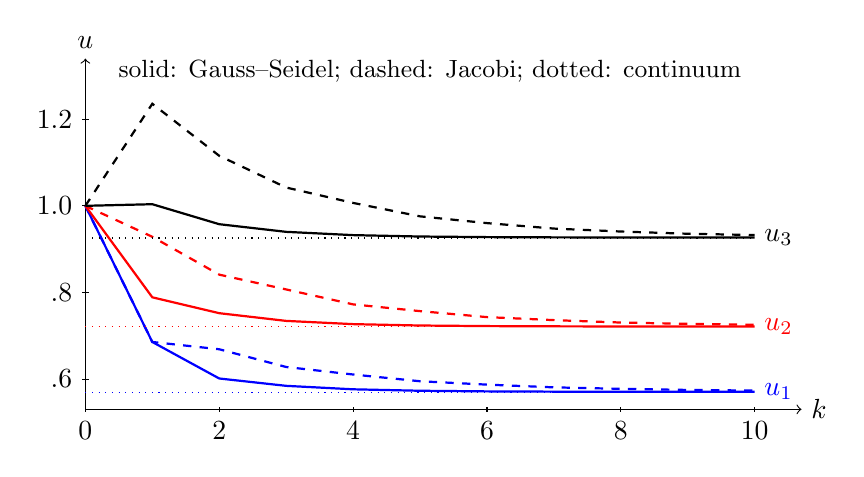
\begin{tikzpicture}[x=.85cm,y=5.5cm]
\draw[->] (0,.53)--(10.7,.53) node[right] {$k$};
\draw[->] (0,.53)--(0,1.34) node[above] {$u$};
\draw[blue,thick,dashed] plot coordinates {(0.000000,1.000000) (1.000000,0.685619) (2.000000,0.668787) (3.000000,0.627836) (4.000000,0.610505) (5.000000,0.594936) (6.000000,0.587145) (7.000000,0.580837) (8.000000,0.577435) (9.000000,0.574853) (10.000000,0.573385)};
\draw[blue,thick] plot coordinates {(0.000000,1.000000) (1.000000,0.685619) (2.000000,0.601303) (3.000000,0.584336) (4.000000,0.576334) (5.000000,0.572964) (6.000000,0.571530) (7.000000,0.570921) (8.000000,0.570662) (9.000000,0.570552) (10.000000,0.570505)};
\draw[blue,dotted] (0,0.5690826)--(10,0.5690826);
\node[blue,right] at (10,0.5704701) {$u_1$};
\draw[red,thick,dashed] plot coordinates {(0.000000,1.000000) (1.000000,0.928466) (2.000000,0.841101) (3.000000,0.806930) (4.000000,0.772450) (5.000000,0.756853) (6.000000,0.743033) (7.000000,0.736106) (8.000000,0.730499) (9.000000,0.727475) (10.000000,0.725180)};
\draw[red,thick] plot coordinates {(0.000000,1.000000) (1.000000,0.788741) (2.000000,0.752098) (3.000000,0.734295) (4.000000,0.726819) (5.000000,0.723637) (6.000000,0.722284) (7.000000,0.721709) (8.000000,0.721465) (9.000000,0.721361) (10.000000,0.721317)};
\draw[red,dotted] (0,0.7204917)--(10,0.7204917);
\node[red,right] at (10,0.7212840) {$u_2$};
\draw[black,thick,dashed] plot coordinates {(0.000000,1.000000) (1.000000,1.235619) (2.000000,1.115516) (3.000000,1.042258) (4.000000,1.006731) (5.000000,0.975681) (6.000000,0.960089) (7.000000,0.947475) (8.000000,0.940671) (9.000000,0.935506) (10.000000,0.932570)};
\draw[black,thick] plot coordinates {(0.000000,1.000000) (1.000000,1.003736) (2.000000,0.957558) (3.000000,0.939923) (4.000000,0.932342) (5.000000,0.929122) (6.000000,0.927753) (7.000000,0.927171) (8.000000,0.926924) (9.000000,0.926818) (10.000000,0.926774)};
\draw[black,dotted] (0,0.9257815)--(10,0.9257815);
\node[black,right] at (10,0.9267407) {$u_3$};
\foreach \k in {0,2,4,6,8,10} \draw (\k,.535)--(\k,.525) node[below] {$\k$};
\foreach \v in {.6,.8,1.0,1.2} \draw (.05,\v)--(-.05,\v) node[left] {$\v$};
\node[anchor=west,font=\small] at (.35,1.31) {solid: Gauss--Seidel; dashed: Jacobi; dotted: continuum};
\end{tikzpicture}

\end{center}
To quantify convergence, write $A=D+L+U$ for the coefficient matrix. Errors
propagate by $B_J=-D^{-1}(L+U)$ and $B_{GS}=-(D+L)^{-1}U$.
Their spectral radii are $0.648377$ and $0.425149$, respectively, explaining
the faster Gauss--Seidel convergence for this update order.
If one instead applies the unreduced nine-point averaging formula literally,
the second Jacobi update is
$b_{k+1}=(8a_k+2b_k+4c_k+s)/20$. That is another valid stationary iteration
with different transient values and the same fixed point; it should not be
mixed with the reduced-system iteration tabulated here.
\end{enumerate}
